% !TEX root = tutor-1-13-2.tex
% Generated tutor view. Edit tasks in task-1-13-2.tex.
\def\TutorEdition{1}
\expandafter\def\csname TutorSourcesdamgia-19657\endcsname{\href{https://phys-ege.sdamgia.ru/problem?id=19657}{Источник: sdamgia-19657}}
\expandafter\def\csname TutorSourcesdamgia-23291\endcsname{\href{https://phys-ege.sdamgia.ru/problem?id=23291}{Источник: sdamgia-23291}}
\expandafter\def\csname TutorSourcesdamgia-23323\endcsname{\href{https://phys-ege.sdamgia.ru/problem?id=23323}{Источник: sdamgia-23323}}
\expandafter\def\csname TutorSourcesdamgia-50852\endcsname{\href{https://phys-ege.sdamgia.ru/problem?id=50852}{Источник: sdamgia-50852}}
\expandafter\def\csname TutorSourcesdamgia-28111\endcsname{\href{https://phys-ege.sdamgia.ru/problem?id=28111}{Источник: sdamgia-28111}}
\expandafter\def\csname TutorSourcesdamgia-24607\endcsname{\href{https://phys-ege.sdamgia.ru/problem?id=24607}{Источник: sdamgia-24607}}
\expandafter\def\csname TutorSourcesdamgia-32080\endcsname{\href{https://phys-ege.sdamgia.ru/problem?id=32080}{Источник: sdamgia-32080}}
% !TEX root = task-1-13-2.tex
% Editable task bank. Append new BankTask blocks at the end of the document.
\documentclass[12pt,a4paper]{article}
\usepackage{physics-textbook}
\usepackage{graphicx,needspace}
\usetikzlibrary{decorations.pathmorphing}
\newif\ifShowSolutions
\ifdefined\TutorEdition
  \ShowSolutionstrue
\else
  \ShowSolutionsfalse % Change to \ShowSolutionstrue to display solutions.
\fi
\newcounter{banktask}
\newsavebox{\BankTaskBox}
\newcommand{\BankTaskContent}[3]{%
  \noindent\textbf{\thebanktask.}\quad #2\par
  \ifShowSolutions
    \Needspace{50mm}% Keep the solution heading with its opening text or diagram.
    #3\par
    \ifdefined\TutorEdition
      \ifcsname TutorSource#1\endcsname
        \nopagebreak\smallskip{\small\csname TutorSource#1\endcsname\par}%
      \fi
    \fi
  \fi
}
\newcommand{\BankTask}[3]{%
  \refstepcounter{banktask}\par\medskip
  \sbox{\BankTaskBox}{\begin{minipage}{\linewidth}%
    \BankTaskContent{#1}{#2}{#3}\end{minipage}}%
  \ifdim\dimexpr\ht\BankTaskBox+\dp\BankTaskBox\relax>\dimexpr\textheight-20mm\relax
    \Needspace{35mm}\BankTaskContent{#1}{#2}{#3}%
  \else
    \Needspace{\dimexpr\ht\BankTaskBox+\dp\BankTaskBox\relax}%
    \noindent\usebox{\BankTaskBox}\par
  \fi
  \medskip
}
\begin{document}
\BookSubsection{1.13.2}{Закон Паскаля}


% Source sdamgia-19657: https://phys-ege.sdamgia.ru/problem?id=19657
\BankTask{sdamgia-19657}{
В герметично закрытую цистерну с плоским дном налит слой воды высотой $5 \,\text{м}$. Над водой находится воздух при атмосферном давлении. Через клапан в крышке цистерны в нее начинают накачивать дополнительные порции воздуха, в результате чего давление воздуха над водой увеличивается в $11{,}5$ раз. Во сколько раз при этом увеличивается давление, которое оказывает содержимое цистерны на ее дно?
}{
\smallskip\noindent\textbf{Решение}\par
Давление, оказываемое на дно цистерны, в первом случае равно $p_{1}=p_{0} + \rho gh,$ во втором случае $p_{2} = 11{,}5p_{0} + \rho gh.$ Учитывая, что $p_{0}=10 ^{5} \,\text{Па},$ получаем:

$\frac{ p_{2}}{ p_{1} } = \frac{ 11{,}5p_{0} + \rho gh}{ p_{0} + \rho gh } = \frac{ 11{,}5 \cdot 10 ^{5} + 10 ^{3} \cdot 10 \cdot 5}{ 10 ^{5} + 10 ^{3} \cdot 10 \cdot 5 } = 8.$

Ответ: $8$.
}

% Source sdamgia-23291: https://phys-ege.sdamgia.ru/problem?id=23291
\BankTask{sdamgia-23291}{
\begin{center}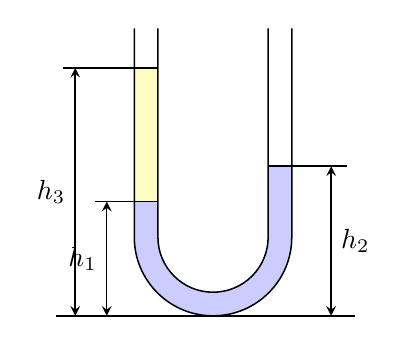
\begin{tikzpicture}[x=1cm,y=1cm,>=stealth,line width=.55pt]
\fill[blue!20] (0,1.1)--(0,.65) arc(180:360:1)--(2,1.55)--(1.7,1.55)--(1.7,.65) arc(0:-180:.7)--(.3,1.1)--cycle;\fill[yellow!25] (0,1.1) rectangle (.3,2.8);\draw (0,3.3)--(0,.65) arc(180:360:1)--(2,3.3);\draw (.3,3.3)--(.3,.65) arc(180:360:.7)--(1.7,3.3);\draw (0,1.1)--(.3,1.1);\draw (0,2.8)--(.3,2.8);\draw (1.7,1.55)--(2,1.55);\draw (-1,-.35)--(2.8,-.35);\draw[<->] (-.75,-.35)--(-.75,2.8) node[midway,left]{$h_3$};\draw (-.9,2.8)--(0,2.8);\draw[<->] (-.35,-.35)--(-.35,1.1) node[midway,left]{$h_1$};\draw (-.5,1.1)--(0,1.1);\draw[<->] (2.5,-.35)--(2.5,1.55) node[midway,right]{$h_2$};\draw (2,1.55)--(2.7,1.55);
\end{tikzpicture}\end{center}
В $U$-образную трубку сначала наливают воду, а затем в одно из колен доливают поверх воды масло. Плотность масла $750 \,\text{кг/м}^3$. Верхний уровень масла находится на высоте $h_{3}=48 \,\text{см}$ от основания трубки, а граница между маслом и водой — на высоте $h_{1}=12 \,\text{см}$. На какой высоте $h_{2}$ находится верхний уровень воды в другом колене трубки?
}{
\smallskip\noindent\textbf{Решение}\par
\begin{center}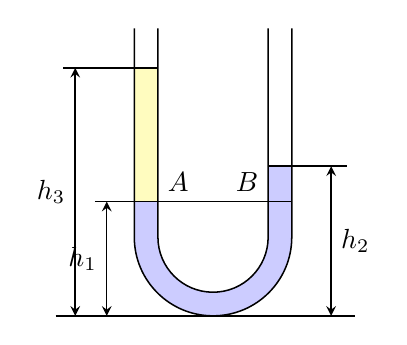
\begin{tikzpicture}[x=1cm,y=1cm,>=stealth,line width=.55pt]
\fill[blue!20] (0,1.1)--(0,.65) arc(180:360:1)--(2,1.55)--(1.7,1.55)--(1.7,.65) arc(0:-180:.7)--(.3,1.1)--cycle;\fill[yellow!25] (0,1.1) rectangle (.3,2.8);\draw (0,3.3)--(0,.65) arc(180:360:1)--(2,3.3);\draw (.3,3.3)--(.3,.65) arc(180:360:.7)--(1.7,3.3);\draw (0,1.1)--(.3,1.1);\draw (0,2.8)--(.3,2.8);\draw (1.7,1.55)--(2,1.55);\draw (-1,-.35)--(2.8,-.35);\draw[<->] (-.75,-.35)--(-.75,2.8) node[midway,left]{$h_3$};\draw (-.9,2.8)--(0,2.8);\draw[<->] (-.35,-.35)--(-.35,1.1) node[midway,left]{$h_1$};\draw (-.5,1.1)--(0,1.1);\draw[<->] (2.5,-.35)--(2.5,1.55) node[midway,right]{$h_2$};\draw (2,1.55)--(2.7,1.55);\draw (0,1.1)--(2,1.1);\node[above right] at (.3,1.1){$A$};\node[above left] at (1.7,1.1){$B$};
\end{tikzpicture}\end{center}

Рассмотрим давление на уровне АВ. Давления жидкости в левом и правом сосудах соответственно равны $p_{A}=\rho_{1}g ( h_{3} - h_{1} ) ,$ $p_{B}=\rho_{2}g ( h_{2} - h_{1} ) .$ По закону Паскаля эти давления равные. 

$\rho_{1}g ( h_{3} - h_{1} ) =\rho_{2}g ( h_{2} - h_{1} ) \Rightarrow$ $h_{2}= \frac{ \rho_{1} ( h_{3} - h_{1} ) + \rho_{2}h_{1}}{ \rho_{2} } = \frac{ 750 \cdot ( 48 - 12 ) + 1000 \cdot 12}{ 1000 } =39\,\text{см}.$

Ответ: $39$.
}

% Source sdamgia-23323: https://phys-ege.sdamgia.ru/problem?id=23323
\BankTask{sdamgia-23323}{
\begin{center}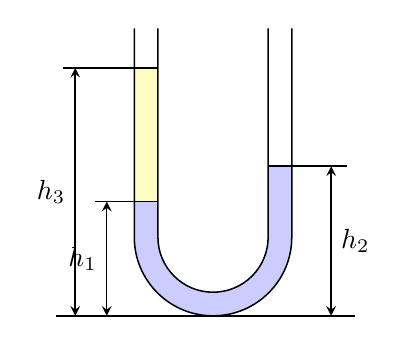
\begin{tikzpicture}[x=1cm,y=1cm,>=stealth,line width=.55pt]
\fill[blue!20] (0,1.1)--(0,.65) arc(180:360:1)--(2,1.55)--(1.7,1.55)--(1.7,.65) arc(0:-180:.7)--(.3,1.1)--cycle;\fill[yellow!25] (0,1.1) rectangle (.3,2.8);\draw (0,3.3)--(0,.65) arc(180:360:1)--(2,3.3);\draw (.3,3.3)--(.3,.65) arc(180:360:.7)--(1.7,3.3);\draw (0,1.1)--(.3,1.1);\draw (0,2.8)--(.3,2.8);\draw (1.7,1.55)--(2,1.55);\draw (-1,-.35)--(2.8,-.35);\draw[<->] (-.75,-.35)--(-.75,2.8) node[midway,left]{$h_3$};\draw (-.9,2.8)--(0,2.8);\draw[<->] (-.35,-.35)--(-.35,1.1) node[midway,left]{$h_1$};\draw (-.5,1.1)--(0,1.1);\draw[<->] (2.5,-.35)--(2.5,1.55) node[midway,right]{$h_2$};\draw (2,1.55)--(2.7,1.55);
\end{tikzpicture}\end{center}
В $U$-образную трубку сначала наливают воду, а затем в одно из колен доливают поверх воды масло. Плотность масла $750 \,\text{кг/м}^3$. Верхний уровень масла находится на высоте $h_{3}=32{,}5 \,\text{см}$ от основания трубки, а верхний уровень воды в другом колене — на высоте $h_{2}=26 \,\text{см}$. На какой высоте $h_{1}$ находится граница между маслом и водой?
}{
\smallskip\noindent\textbf{Решение}\par
\begin{center}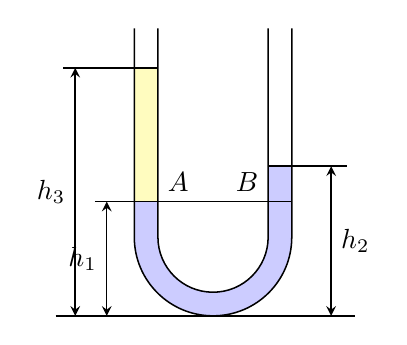
\begin{tikzpicture}[x=1cm,y=1cm,>=stealth,line width=.55pt]
\fill[blue!20] (0,1.1)--(0,.65) arc(180:360:1)--(2,1.55)--(1.7,1.55)--(1.7,.65) arc(0:-180:.7)--(.3,1.1)--cycle;\fill[yellow!25] (0,1.1) rectangle (.3,2.8);\draw (0,3.3)--(0,.65) arc(180:360:1)--(2,3.3);\draw (.3,3.3)--(.3,.65) arc(180:360:.7)--(1.7,3.3);\draw (0,1.1)--(.3,1.1);\draw (0,2.8)--(.3,2.8);\draw (1.7,1.55)--(2,1.55);\draw (-1,-.35)--(2.8,-.35);\draw[<->] (-.75,-.35)--(-.75,2.8) node[midway,left]{$h_3$};\draw (-.9,2.8)--(0,2.8);\draw[<->] (-.35,-.35)--(-.35,1.1) node[midway,left]{$h_1$};\draw (-.5,1.1)--(0,1.1);\draw[<->] (2.5,-.35)--(2.5,1.55) node[midway,right]{$h_2$};\draw (2,1.55)--(2.7,1.55);\draw (0,1.1)--(2,1.1);\node[above right] at (.3,1.1){$A$};\node[above left] at (1.7,1.1){$B$};
\end{tikzpicture}\end{center}

Рассмотрим давление на уровне АВ. Давления жидкости в левом и правом сосудах соответственно равны $p_{A}=\rho_{1}g ( h_{3} - h_{1} ) ,$ $p_{B}=\rho_{2}g ( h_{2} - h_{1} ) .$ По закону Паскаля эти давления равные. 

$\rho_{1}g ( h_{3} - h_{1} ) =\rho_{2}g ( h_{2} - h_{1} ) \Rightarrow$ $h_{1}= \frac{ \rho_{\text{в}}h_{2} - \rho_{\text{м}}h_{3}}{ \rho_{\text{в}} - \rho_{\text{м}} } = \frac{ 1000 \cdot 26 - 750 \cdot 32{,}5}{ 1000 - 750 } =6{,}5\,\text{см}.$

Ответ: $6{,}5$.
}

% Source sdamgia-50852: https://phys-ege.sdamgia.ru/problem?id=50852
\BankTask{sdamgia-50852}{
\begin{center}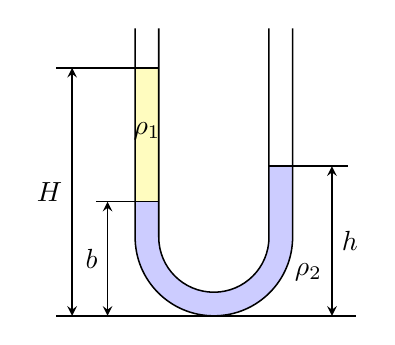
\begin{tikzpicture}[x=1cm,y=1cm,>=stealth,line width=.55pt]
\fill[blue!20] (0,1.1)--(0,.65) arc(180:360:1)--(2,1.55)--(1.7,1.55)--(1.7,.65) arc(0:-180:.7)--(.3,1.1)--cycle;\fill[yellow!25] (0,1.1) rectangle (.3,2.8);\draw (0,3.3)--(0,.65) arc(180:360:1)--(2,3.3);\draw (.3,3.3)--(.3,.65) arc(180:360:.7)--(1.7,3.3);\draw (0,1.1)--(.3,1.1);\draw (0,2.8)--(.3,2.8);\draw (1.7,1.55)--(2,1.55);\draw (-1,-.35)--(2.8,-.35);\node at (.15,2){$\rho_1$};\node at (2.2,.2){$\rho_2$};\draw[<->] (-.8,-.35)--(-.8,2.8) node[midway,left]{$H$};\draw (-1,2.8)--(0,2.8);\draw[<->] (-.35,-.35)--(-.35,1.1) node[midway,left]{$b$};\draw (-.5,1.1)--(0,1.1);\draw[<->] (2.5,-.35)--(2.5,1.55) node[midway,right]{$h$};\draw (2,1.55)--(2.7,1.55);
\end{tikzpicture}\end{center}

В широкую $U$-образную трубку с вертикальными прямыми коленами налиты неизвестная жидкость плотностью $\rho _{1}$ и вода плотностью $\rho_{2}= 1{,}0 \cdot 10 ^{3} \,\text{кг/м} ^{3}$ (см. рис.). На рисунке $b = 10\,\text{см},$ $h= 24\,\text{см},$ $H = 30\,\text{см}.$ Какова плотность жидкости $\rho _{1}$?
}{
\smallskip\noindent\textbf{Решение}\par
Поскольку жидкости в $U$-образной трубке статичны, приравняем давления воды на высоте $b$ от земли в правом и левом коленах:

$p_{\text{лев}}=p_{\text{прав}} \Longleftrightarrow p_{\text{атм}} + \rho_{1} g ( H - b ) = p_{\text{атм}} + \rho_{2} g ( h - b ) \Longleftrightarrow$
 
$\Longleftrightarrow \rho_{1}=\rho_{2} \frac{ h - b}{ H - b } =1 \cdot 10 ^{3} \,\text{кг/м} ^{3} \cdot \frac{ 24\,\text{см} - 10\,\text{см}}{ 30\,\text{см} - 10\,\text{см} } =0{,}7 \cdot 10 ^{3} \,\text{кг/м} ^{3} =700\,\text{кг/м} ^{3} .$

Ответ: $700$.
}

% Source sdamgia-28111: https://phys-ege.sdamgia.ru/problem?id=28111
\BankTask{sdamgia-28111}{
\begin{center}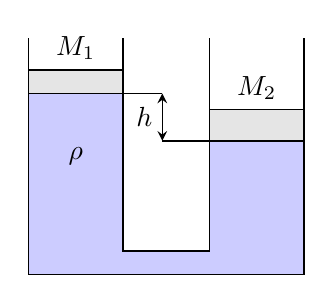
\begin{tikzpicture}[x=1cm,y=1cm,>=stealth,line width=.55pt]
\fill[blue!20](0,2.3)--(1.2,2.3)--(1.2,.3)--(2.3,.3)--(2.3,1.7)--(3.5,1.7)--(3.5,0)--(0,0)--cycle;\draw(0,3)--(0,0)--(3.5,0)--(3.5,3);\draw(1.2,3)--(1.2,.3)--(2.3,.3)--(2.3,3);\draw[fill=gray!20](0,2.3)rectangle(1.2,2.6);\draw[fill=gray!20](2.3,1.7)rectangle(3.5,2.1);\node[above]at(.6,2.6){$M_1$};\node[above]at(2.9,2.1){$M_2$};\node at(.6,1.5){$\rho$};\draw(1.2,2.3)--(1.7,2.3);\draw(1.7,1.7)--(2.3,1.7);\draw[<->](1.7,1.7)--(1.7,2.3)node[midway,left]{$h$};
\end{tikzpicture}\end{center}
Два одинаковых вертикальных сообщающихся цилиндрических сосуда заполнены водой и закрыты поршнями массами $M_{1}=1 \,\text{кг}$ и $M_{2}=2 \,\text{кг}$. Когда система находится в равновесии, правый поршень с площадью основания $100 \,\text{см}^2$ расположен ниже левого на величину $h=10 \,\text{см}$.

 
\par\smallskip\noindent $1$. Величина $h$ при заданных массах поршней зависит от плотности материала, из которого они изготовлены.
\par\smallskip\noindent $2$. Если на левый поршень поместить груз массой $m=1 \,\text{кг}$, поршни будут находиться на одном уровне.
\par\smallskip\noindent $3$. Если на правый поршень поместить груз массой $m=1 \,\text{кг}$, разность уровней между левым и правым поршнями составит $15 \,\text{см}$.
\par\smallskip\noindent $4$. Если массу левого поршня увеличить на $1 \,\text{кг}$, то он сдвинется на $5 \,\text{см}$ вниз.
\par\smallskip\noindent $5$. Если вместо воды в сосуды налить керосин, то в состоянии равновесия левый поршень будет выше правого на $12{,}5 \,\text{см}$.
}{
\smallskip\noindent\textbf{Решение}\par
\par\smallskip\noindent $1$. Неверно. Величина высоты $h$ зависит от массы каждого поршня. Так как в условии не сказано об объемах поршней, то невозможно судить о плотностях материала, из которого они изготовлены.
\par\smallskip\noindent $2$. Верно. В начальный момент времени система находилась в равновесии. Следовательно:

$\frac{ M_{1}g}{ S } + \rho gh= \frac{ M_{2}g}{ S } .$

Когда на левый поршень положили груз, условие равновесия приобрело вид:

$\frac{ ( M_{1} + m ) g}{ S } + \rho gh_{1}= \frac{ M_{2}g}{ S } .$

Отсюда получаем, что $h - h_{1}=10\,\text{см}.$ Учитывая, что $h=10 \,\text{см}$, делаем вывод, что $h_{1}=0$, значит, поршни находятся на одном уровне.
\par\smallskip\noindent $3$. Неверно. Условие равновесия в случае, когда на правый поршень положили груз $m=1 \,\text{кг}$, имеет вид:

$\frac{ M_{1}g}{ S } + \rho gh_{1}= \frac{ ( M_{2} + m ) g}{ S } ,$
 откуда $h_1-h=10\,\text{см}$.
\par\smallskip\noindent $4$. Верно. Если массу левого поршня увеличить на $1 \,\text{кг}$, то поршни будут находиться на одном уровне (следует из рассуждений пункта $2$).
\par\smallskip\noindent $5$. Верно. Из уравнения равновесия 

$\frac{ M_{1}g}{ S } + \rho gh= \frac{ M_{2}g}{ S }$
 
разность уровней определяется:

$h= \frac{ M_{2} - M_{1}}{ \rho S } = \frac{ 2 - 1}{ 800 \cdot 10 ^{ - 2 } } =0{,}125\,\text{м} =12{,}5\,\text{см}.$

Ответ: $245$.
}

% Source sdamgia-24607: https://phys-ege.sdamgia.ru/problem?id=24607
\BankTask{sdamgia-24607}{
\begin{center}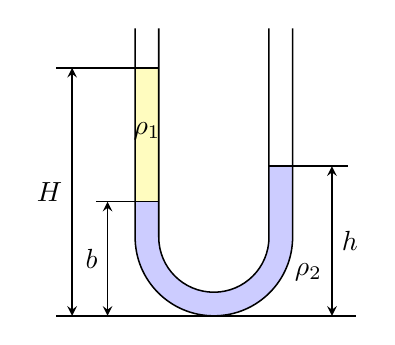
\begin{tikzpicture}[x=1cm,y=1cm,>=stealth,line width=.55pt]
\fill[blue!20] (0,1.1)--(0,.65) arc(180:360:1)--(2,1.55)--(1.7,1.55)--(1.7,.65) arc(0:-180:.7)--(.3,1.1)--cycle;\fill[yellow!25] (0,1.1) rectangle (.3,2.8);\draw (0,3.3)--(0,.65) arc(180:360:1)--(2,3.3);\draw (.3,3.3)--(.3,.65) arc(180:360:.7)--(1.7,3.3);\draw (0,1.1)--(.3,1.1);\draw (0,2.8)--(.3,2.8);\draw (1.7,1.55)--(2,1.55);\draw (-1,-.35)--(2.8,-.35);\node at (.15,2){$\rho_1$};\node at (2.2,.2){$\rho_2$};\draw[<->] (-.8,-.35)--(-.8,2.8) node[midway,left]{$H$};\draw (-1,2.8)--(0,2.8);\draw[<->] (-.35,-.35)--(-.35,1.1) node[midway,left]{$b$};\draw (-.5,1.1)--(0,1.1);\draw[<->] (2.5,-.35)--(2.5,1.55) node[midway,right]{$h$};\draw (2,1.55)--(2.7,1.55);
\end{tikzpicture}\end{center}
В широкую $U$-образную трубку с вертикальными прямыми коленами налиты керосин и вода (см. рис.). На рисунке $b=10 \,\text{см}$, $H=30 \,\text{см}$. Какова высота жидкости в правом колене?
}{
\smallskip\noindent\textbf{Решение}\par
\par\smallskip\noindent $1$. Рассмотрим давление жидкостей в обоих коленах на уровне границы жидкостей. По закону Паскаля давление в обоих коленах на этом уровне должно быть одинаковым.
\par\smallskip\noindent $2$. Поскольку высота столба жидкости в левом колене больше, чем в правом, делаем вывод, что в левом колене плотность жидкости меньше, чем в правом, то есть в левом — керосин, в правом — вода. Давление жидкости в левом колене равно $p_{1}=\rho_{1}g ( H - b ) + p_{a},$ в правом колене равно $p_{2}=\rho_{2}g ( h - b ) + p_{a}.$ Из равенства давлений получаем: 

$h= \frac{ \rho_{1} ( H - b ) }{ \rho_{2} } + b= \frac{ 800 \cdot ( 30 - 10 ) }{ 1000 } + 10=26\,\text{см}.$

Ответ: $26 \,\text{см}$.
}

% Source sdamgia-32080: https://phys-ege.sdamgia.ru/problem?id=32080
\BankTask{sdamgia-32080}{
\begin{center}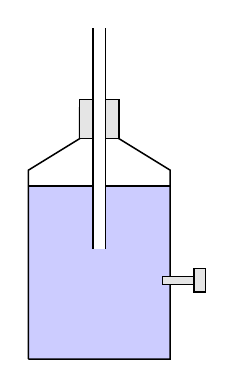
\begin{tikzpicture}[x=1cm,y=1cm,>=stealth,line width=.55pt]
\fill[blue!20] (0,0) rectangle (1.8,2.2);\draw (0,0)--(0,2.4)--(.65,2.8)--(.65,3.2);\draw (1.15,3.2)--(1.15,2.8)--(1.8,2.4)--(1.8,0)--(0,0);\draw (0,2.2)--(1.8,2.2);\draw[fill=gray!20] (.65,2.8) rectangle (1.15,3.3);\fill[white] (.82,1.4) rectangle (.98,4.2);\draw (.82,1.4)--(.82,4.2);\draw (.98,1.4)--(.98,4.2);\draw[fill=gray!20] (1.7,.95) rectangle (2.1,1.05);\draw[fill=gray!20] (2.1,.85) rectangle (2.25,1.15);
\end{tikzpicture}\end{center}
В боковой стенке покоящейся на столе бутылки проделано маленькое отверстие, в которое вставлена затычка. В бутылку налита вода, а горлышко бутылки закрыто резиновой пробкой, через которую пропущена вертикальная тонкая трубка. Нижний конец трубки находится выше отверстия в стенке бутылки, но ниже поверхности воды, а верхний конец сообщается с атмосферой (см. рис.). Затычку из отверстия в боковой стенке вынимают, и вода вытекает из бутылки через отверстие. При этом через трубку в бутылку входят пузырьки воздуха. Затем трубку начинают медленно опускать вниз и делают это до тех пор, пока нижний конец трубки не окажется на одном уровне с отверстием.
Опишите, как будет изменяться скорость вытекания воды из отверстия по мере опускания трубки. Считайте, что уровень воды всегда находится выше нижнего конца трубки и выше отверстия в стенке. Ответ обоснуйте, указав, какие физические закономерности Вы использовали для объяснения.
}{
\smallskip\noindent\textbf{Решение}\par
\begin{center}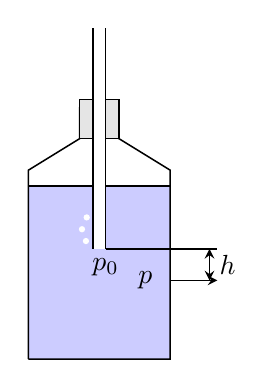
\begin{tikzpicture}[x=1cm,y=1cm,>=stealth,line width=.55pt]
\fill[blue!20] (0,0) rectangle (1.8,2.2);\draw (0,0)--(0,2.4)--(.65,2.8)--(.65,3.2);\draw (1.15,3.2)--(1.15,2.8)--(1.8,2.4)--(1.8,0)--(0,0);\draw (0,2.2)--(1.8,2.2);\draw[fill=gray!20] (.65,2.8) rectangle (1.15,3.3);\fill[white] (.82,1.4) rectangle (.98,4.2);\draw (.82,1.4)--(.82,4.2);\draw (.98,1.4)--(.98,4.2);\fill[white] (.73,1.5) circle(.04);\fill[white] (.68,1.65) circle(.04);\fill[white] (.74,1.8) circle(.04);\draw[->] (1.8,1)--(2.4,1);\draw (.98,1.4)--(2.4,1.4);\draw[<->] (2.3,1)--(2.3,1.4) node[midway,right]{$h$};\node[below] at (.98,1.4){$p_0$};\node[left] at (1.7,1){$p$};
\end{tikzpicture}\end{center}
\par\smallskip\noindent $1$) При вытекании воды из отверстия в бутылке в нее через трубку входят пузырьки воздуха. Это означает, что давление в жидкости на уровне нижнего конца трубки равно атмосферному давлению $p_{0}.$ На уровне отверстия в боковой стенке, которое находится ниже конца трубки на величину $h$, давление в жидкости равно $p = p_{0} + \rho gh,$ где $\rho$ — плотность воды. Это следует из закона Паскаля и из формулы для давления в жидкости, покоящейся в ИСО в однородном поле силы тяжести.
\par\smallskip\noindent $2$. Скорость вытекания воды из отверстия определяется разностью давлений внутри и снаружи сосуда на уровне отверстия в стенке: $\Delta p = p - p_{0} = \rho gh,$ то есть зависит только от $h$. Поэтому при неподвижной трубке скорость вытекания будет постоянной.
\par\smallskip\noindent $3$. Если опускать трубку, разность высот $h$ будет уменьшаться, а значит, будут уменьшаться разность давлений $\Delta p$ и зависящая от нее скорость вытекания воды. Поэтому при опускании трубки вода будет вытекать из отверстия все медленнее и медленнее. Когда нижний конец трубки окажется на одном уровне с отверстием, давление внутри воды в бутылке на этом уровне станет равно атмосферному, и вода перестанет вытекать из бутылки.
}

\end{document}

